\documentclass[letter,11pt]{article}
\usepackage[breaklinks]{hyperref}
\hypersetup{
    bookmarks=true,         % show bookmarks bar?
    unicode=false,          % non-Latin characters in Acrobat’s bookmarks
    pdftoolbar=true,        % show Acrobat’s toolbar?
    pdfmenubar=true,        % show Acrobat’s menu?
    pdffitwindow=false,     % window fit to page when opened
    pdfstartview={XYZ null null 1.00},    % disable zoom
    pdftitle={Final Exam Review},    % title
    pdfauthor={Richard Zak},     % author
    pdfsubject={UMBC CMSC104 Problem Solving and Computer Programming},   % subject of the document
    pdfkeywords={Computer Science, Programming, Problem Solving, CSEE}, % list of keywords
    pdfnewwindow=true,      % links in new PDF window
    colorlinks=false,       % false: boxed links; true: colored links
    linkcolor=red,          % color of internal links (change box color with linkbordercolor)
    citecolor=green,        % color of links to bibliography
    filecolor=magenta,      % color of file links
    urlcolor=cyan           % color of external links
}
\usepackage{graphicx}
\usepackage{fancyhdr}
\usepackage{multicol}
\pagestyle{fancy}
\usepackage[letterpaper, margin=1in]{geometry}
\geometry{letterpaper}
\usepackage{parskip} % Disable initial indent
\usepackage{color,soul} % Highligher
\usepackage[normalem]{ulem} % Strikethrough with \sout{}
\usepackage{placeins} % FloatBarrier
\usepackage[utf8]{inputenc}

% arrays table
\usepackage{multirow,tabularx}
\newcolumntype{Y}{>{\centering\arraybackslash}X}
\renewcommand{\arraystretch}{2}

\fancyhf{}
\renewcommand{\headrulewidth}{0pt} % Remove default underline from header package
\rhead{CMSC 104 Section 01: Final Exam Review}
%\rhead{}
\lhead{\begin{picture}(0,0) \put(0,-10){
\includegraphics[width=1.1cm]{Images/UMBC-vertical}} \end{picture}}
\cfoot{\thepage}
\rfoot{Spring 2024}
\lfoot{CMSC 104 Section 01}
\AtEndDocument{\vfill \footnotesize{Last modified: 07 December 2021}}
\AtEndDocument{\rfoot{Spring 2024}}
\renewcommand\thesubsection{\arabic{subsection}} % Show only subsection numbers, not section.subsection
\title{Final Exam Review}

\begin{document}
%\maketitle
\huge
\textbf{Final Exam Review}
\normalsize

\tableofcontents

\section{Computer Components}
\paragraph{}A computer is a device which performs computation on numbers. It is through the meaning we give those numbers that data is represented and ultimately useful. A computer takes many forms: cell phones, laptops, desktops, servers, control systems in automobiles \& aircraft, video game consoles, smart watches, and many more. They vary drastically in price, from a \$35 Raspberry Pi\footnote{Raspberry Pi website: \url{https://www.raspberrypi.org/}}, which is about the size of a credit card and geared for students \& hobbyists, to multi-million dollar government-operated supercomputers\footnote{\url{https://en.wikipedia.org/wiki/Supercomputer}}.

\subsection{Storage}
\paragraph{}Storage on a computer is thought of as long or short-term storage.
\begin{itemize}
    \item Short-term (or ephemeral) storage: \hyperref[sec:ram]{RAM} is gone when the computer turns off.
    \item Long-term (or permanent) storage: hard drives, removable media, and other devices which hold data even when the computer is powered off, or when removed from the computer.
\end{itemize}

\paragraph{}Long-term storage can be a hard drive, USB thumb drive, CD or DVD optical disc, floppy disks, or tape back-up systems. \textit{Short-term storage (memory) is ALWAYS faster}, and the long-term storage devices are ranked from fastest to slowest:
\begin{enumerate}
    \item Hard drive (solid state, or SSD)
    \item Hard drive (spinning magnetic disk, or HDD)
    \item USB thumb drive
    \item CD or DVD optical drive
    \item Tape
\end{enumerate}

\paragraph{}Computer memory and these long-term storage devices provide \texttt{random access}, meaning it is possible to read any single byte from any location without having to read \texttt{all} of the preceding bytes. The exception: tape back-up. To retrieve some data at the end of the tape, the entirety of the tape's contents must be read! This, and because the tape systems are slow, makes reading from tape data very slow.

\subsection{Input/Output Devices}
\paragraph{}Simply put, input devices receive data, and output devices send data to the user. Examples:
\begin{itemize}
    \item Input: keyboard, mouse, scanner, webcam
    \item Output: monitor, graphics card, printer
    \item Input \& Output: network card, audio card (audio out to speakers, microphone input), USB devices
\end{itemize}

\subsection{Busses}
\paragraph{}A bus is a mechanism for handling communications between many components. The most common example is USB (which stands for Universal Serial Bus). The USB hardware in the computer handles all the communications for the many USB devices which may be plugged in to the computer.

\paragraph{}Another example is the PCI bus, which connects the various cards inside most desktop and server systems, most commonly a graphics card in gaming systems.

\paragraph{}In general, the bus has many wires for communicating data to and from the various devices, ensuring that the data gets to the proper destination without error.

\subsection{Central Processing Unit (CPU)}
\paragraph{}Made up of billions of transistors yet taking up less space than a fingernail, the modern CPU can be thought of as the ``brain'' of the computer. It provides instruction to the rest of the devices, and ensures that the devices communicate with each other.

\paragraph{}Processors have memory of their own, called registers and cache. These are the fastest forms of memory on a computer, though management of this memory is solely managed by the processor itself.

\subsection{Random Access Memory}\label{sec:ram}
\paragraph{}System memory is in the form of memory sticks connected to the motherboard, sometimes permanently connected. These circuits are fast, temporary storage, and are used by the operating system to keep the computer running, and by running applications to perform the tasks asked of them. More RAM in a computer generally makes the computer \texttt{seem} faster, as more things can be done without having to temporarily save data to disk. This is done so that the computer may function even when the system memory is exhausted, but since hard drives are much slower than RAM, it seems to take longer to use applications when this happens.

\section{Operating Systems}
\paragraph{}The operating system is a program which manages the computer's functionality on behalf of the user, and is the user's interface to the hardware. The operating system manages the devices to ensure sound comes out of the speakers from a music player, for example. The two main types of operating systems, with their respective sub-types:
\begin{itemize}
    \item Windows
    \item Unix or Unix-like
    \begin{itemize}
        \item macOS (including iOS, iPadOS, etc)
        \item Linux
        \begin{itemize}
            \item Android
        \end{itemize}
        \item FreeBSD, OpenBSD, NetBSD
        \item Solaris
        \item AIX
    \end{itemize}
\end{itemize}

\subsection{Unix Commands}
\paragraph{}Some basic Unix commands, which usually work across Unix and Unix-like operating systems:
\begin{itemize}
    \item \texttt{cat <fileName>}: Show the contents of a file, followed by the path to that file
    \item \texttt{cd <dirName>}: Change directory, followed by the directory path to change to
    \item \texttt{ls}: List the contents of a directory
    \item \texttt{mv from/path/A to/path/B}: Move a file (or directory) from location A to location B
    \item \texttt{pwd}: print working directory (current location)
    \item \texttt{rm filename}: Remove (delete) a file or directory (\texttt{rm -r dirName})
\end{itemize}

\FloatBarrier
\section{Number Formats}
\paragraph{}Numbers are written out according to their base. The numbers we typically use are in base 10, that is, they range from zero to nine, then start again with a new number in front, so 9 becomes 10, for example. Another example is how we tell time during the day using base 60. Fifty nine minutes plus one becomes 1 hour and zero minutes.

\paragraph{Binary}Each part of memory in a computer is basically a switch, it's either off (zero) or on (one). Since there are only two states, this is base 2, and this is how data is represented in memory and in the CPU.

\paragraph{Decimal}This is base 10, the number system we are familiar using.

\paragraph{Octal}This is base 8, using the numbers zero though 7. These numbers are often written with a capital ``O'' preceding the number, or with a subscript 8 after the number (a O can be difficult to distinguish from a 0).

\paragraph{Hexadecimal}Very quickly, binary numbers get very large, especially when dealing with computer memory. To make this easier, hexadecimal is often used. This is base 16, using the letters A-F to represent 10-15. These numbers are often written with ``0x'' preceding the number, or with ``h'' after the number.

\begin{figure}[h!]
    \centering
    \begin{tabular}{l l}
         Binary:      & 1 1 0 1 0 0 0 0 1 0 1 0 0 1 1 1  \\
         Octal:       & $150247_8$ (or O150247) \\
         Decimal:     & $53414_{10}$ \\
         Hexadecimal: & $D0A7_{16}$ (or 0xD0A7, or D0A7h)
    \end{tabular}
    \caption{The same number in different formats}
    \label{fig:datatypesequivalent}
\end{figure}

\subsection{Decimal and Binary to Hex}
\paragraph{}Converting between binary and hexadecimal can be done directly. Starting from the right, four bits can be directly converted to hexadecimal. See \autoref{fig:binhexfig} for an example, source: \url{https://owlcation.com/stem/How-to-Convert-Hex-to-Binary-and-Binary-to-Hexadecimal}.

\begin{figure}[h!]
    \centering
    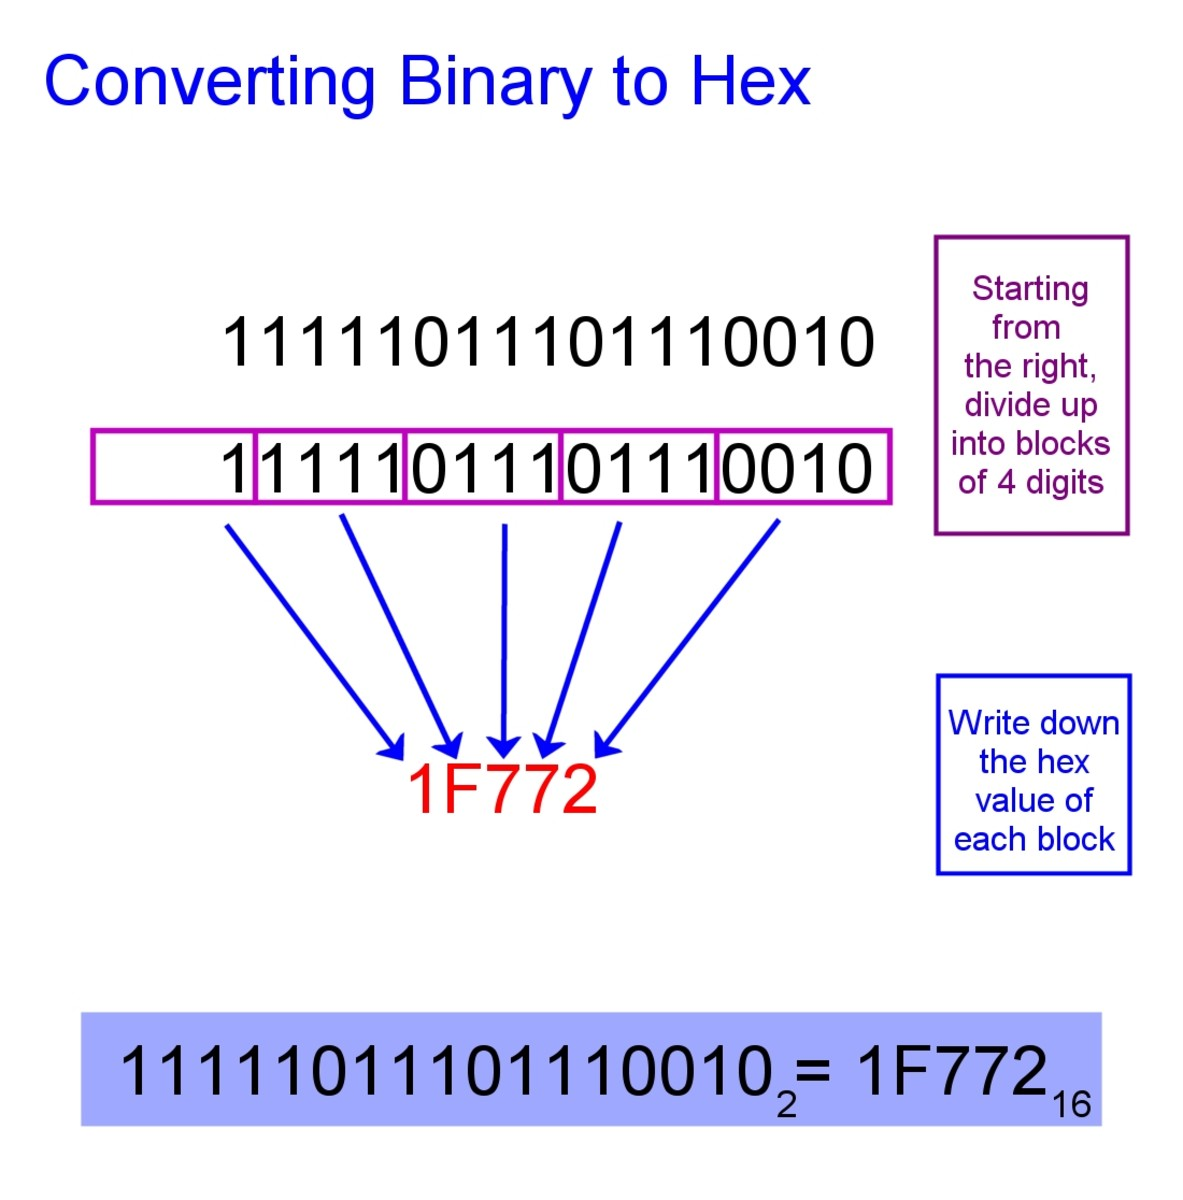
\includegraphics[scale=0.31]{FinalExam/bin_hex.jpg}
    \caption{Binary to Hex}
    \label{fig:binhexfig}
\end{figure}
\FloatBarrier

\section{Semantics vs Syntax}
\paragraph{Semantics} The meaning or purpose of a phrase, sentence, of segment of code is referred to as semantics. Example: \textit{The dog caught the ball} vs. \textit{The ball walked the dog.}. The second example doesn't make sense.

\paragraph{Syntax} The manner in which code or human language is structured is syntax. Example: \textit{The dog caught the ball.} vs. \textit{dog ball caught the the}.

\paragraph{}Semantics vs. syntax are based on the language. A pattern used by one language won't likely be valid for another language, and the same is true of programming languages.

\paragraph{Note:}The compiler will catch syntax errors. Semantic errors, also sometimes called bugs\footnote{Computer bugs got their name from a time in September 1947, where a computer problem was caused by an actual insect. \url{https://www.atlasobscura.com/places/grace-hoppers-bug}.}, are not caught automatically. You have to identify them, and figure out how to resolve them. If someone could invent a semantic error detector which works with a compiler, that person would be a billionaire.

\section{Algorithms}
\paragraph{}An algorithm is a set of instructions which is clear \& easy to understand no matter who reads it, and has a small (or manageable) amount of steps. It is clear at each step what must be done, without assumptions.

\paragraph{}A professor at Havard University made a vdeo which demonstrates this clearly by discussing how to make a peanut butter and jelly sandwich: \url{https://youtu.be/okkIyWhN0iQ}. Note that some steps, like ``open the bag'', or how to open the bag of bread, is missed because some people \textit{assumed} that step based on prior knowledge. A good algorithm wouldn't have an assumption, each step would be clear. If an assumption can't be avoided, it would be documented somewhere in the code.

\section{Pseudocode}
\paragraph{}To help with planning how a program, or function might look like, \texttt{pseudocode} is used because it hides the issues pertaining to C syntax. Separating out semantics from syntax can be helpful in planning how the code will look by first focusing on what it's supposed to do. Example:

\begin{verbatim}
    DISPLAY "How many grades?"
    READ <numberOfGrades>
    counter = 0
    sum = 0
    WHILE (<counter> < <numberOfGrades>)
        READ <grade>
        <sum> = <sum> + <grade>
    END_WHILE
    average = <sum> / <numberOfGrades>
    DISPLAY "Class average", <average>
\end{verbatim}

\section{Programming in C}
\paragraph{}C is an exciting and powerful programming language. It's been used to create operating systems, video games, web browsers, word processors, and to program some microchips (like Arduino\footnote{\url{https://www.arduino.cc/}}).

\subsection{Compiling}
\paragraph{}Compiling is the process of converting typed programming language code into an executable file which can be run by the operating system. The program which makes this conversion is a \texttt{compiler}, and it operates at three stages:
\begin{enumerate}
    \item Preprocessing: handing all the lines of code which start with ``\#''.
    \item Compiling: turning the code into machine code, syntax errors are caught here.
    \item Linking: connecting the code with external libraries, so the operating system can run it.
\end{enumerate}

\subsection{Variables}
\paragraph{}Like in math, C has variables which have a data type, and a name. For example, \texttt{int temp = 5;} declares an integer variable called ``temp'', and sets its initial value to five. The data type could have been something different, but once set, it will always be that type. An integer can't hold a floating point number, for example.

\subsection{Order of Operations}
\begin{figure}[h!]
    \centering
    \begin{tabular}{l l}
        Precedence & Associativity \\ \hline
        ( ) & left to right/inside-out \\
        * / \% & left to right \\
        + (addition) - (subtraction) & left to right \\
        $<$ $<=$ $>$ $>=$ & left to right \\
        == != & left to right \\
        \&\& & left to right \\
        \textbar\textbar & left to right \\
        $=$ & right to left
    \end{tabular}
    \caption{Operator Precedence}
    \label{fig:opprec}
\end{figure}

\FloatBarrier
\subsection{Data Types}\label{sec:datatypes}
\paragraph{}The computer only knows about numbers, nothing else. Data types are the lens by which we view those numbers, giving them meaning. Data types have different sizes, which determines their maximum and minimum sizes. When writing code, it's important to ensure that the proper data type is chosen. The data type should be large enough to accommodate the data which will be processed, but not wasteful of computer memory.
\begin{figure}[h!]
    \centering
    \begin{tabular}{lcll}
        Type           & Size & Minimum & Maximum \\ \hline
        char           & 1    & -127    & +128 \\
        unsigned char  & 1    & 0       & +255 \\
        short          & 2    & -32,767 & +32,767   \\
        unsigned short & 2    & 0       & +65,535 \\
        int            & 4    & -2,147,483,647 & +2,147,483,647 \\
        unsigned int   & 4    & 0              & +4,294,967,295 \\
        long           & 8    & -9 quintillion & + 9 quintillion \\
        unsigned long  & 8    & 0              & +18 quintillion \\
        float          & 4    & 1.175494351 E-38  & 3.402823466 E +38 \\
        double         & 8    & 2.225073858 E-308 & 1.797693135 E +308
    \end{tabular}
    \caption{Data Types: Sizes, Value Range}
    \label{fig:datatypeschart}
\end{figure}

\paragraph{}For a program calculating or using the distance to Voyager 1 in astronomical units, then use an integer: \texttt{int distToVoyagerAU = 156;}. If the distance to Voyager 1 would be needed in inches, use a float: 
\begin{verbatim}
    #include <math.h> // so we can use exponents

    float distToVoyagerInches = 9.16 * powf(10, 14);
\end{verbatim}

\paragraph{}It's a silly example, but $9.6 x 10^{14}$ is less than the maximum of $10^{38}$. But if operations are to be done which modify that variable, potentially make it bigger by consider using a \texttt{double} instead.

\FloatBarrier
\subsubsection{ASCII Table}
\paragraph{}Since the computer can only understand numbers, characters and character arrays (also known as strings) exist in memory as integers. The ASCII table shows the mapping of integer value to character. The full table is shown in \autoref{fig:asciitable}, from \url{https://www.asciitable.com/}.

\begin{figure}[h!]
    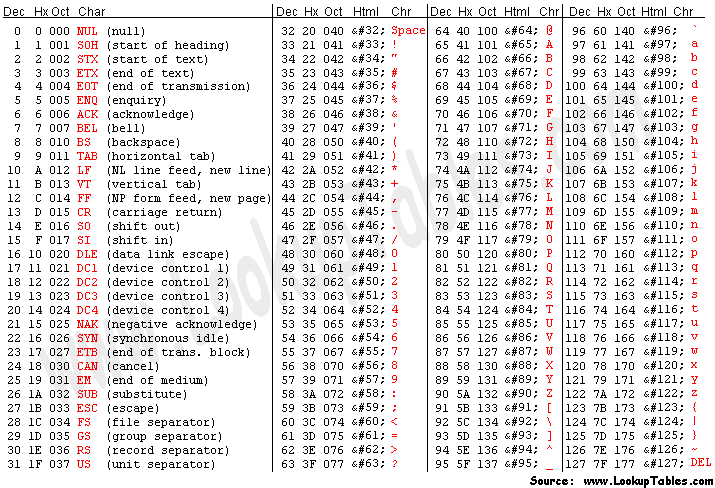
\includegraphics[scale=0.72]{FinalExam/asciifull.png}
    \caption{ASCII Table from asciitable.com}
    \label{fig:asciitable}
\end{figure}

\FloatBarrier
\subsection{Loops}
\paragraph{}Loops are useful, in that they allow doing the same thing several times without typing everything out. There are three different types of loops designed to be used in different circumstances. Each instance of the loop doing some task is an \textit{iteration}.
\begin{itemize}
    \item \texttt{while}: A while loop runs zero or many times, used when the number of iterations is not known (event-based).
    \item \texttt{for}: A for loop runs for zero or many times, used when the number of iterations is known in advance (counter-based).
    \item \texttt{do...while}: A do while loop runs for one or many times, used when the number if iterations is not known, but will be at least once (event-based). This is useful for handling input with error checking, for example.
\end{itemize}

\subsection{If Statements}
\paragraph{}If statements are an example of binary selection, either \textit{this} or \textit{that}.
\begin{verbatim}
if (tempVar == 12) {
    doThis();
} else {
    doThat();
}
\end{verbatim}

\subsection{Switch \& Case Statements}
\paragraph{}In some scenarios, it is necessary to chose some action based on a wide possible set of values. Instead of having nested \texttt{if} statements, a \texttt{switch} statement can be used where the variable being used is an \texttt{integer} or \texttt{char}. The \texttt{default} statement is usually used to handle errors, when the value used for the \texttt{switch} statement wasn't expected, or is invalid.

\paragraph{}The \texttt{case} statement has the value for that statement, and usually each \texttt{case} statement ends with \texttt{break;}. Sometimes, it makes sense to have the \texttt{case} statement \textit{cascade} down to the next \texttt{case} statement, if the action to be done for those values would be the same.

\begin{verbatim}
int tempVar = doSomething();
switch tempVar {
    case 1: doSomething(); break;
    case 2: doSomethingElse() break;
    case 3: doEvenSomethingElse(); break;
    case 4:
    case 5: nowForSomethingCompletelyDifferent(); break;
    default: printf("Invalid value: %d\n", tempVar);
}
\end{verbatim}

\subsection{Operators}

\subsubsection{Unary Operators}
\paragraph{}Unary operators have only one argument: the variable they are modifying. If the operator comes before the variable, then the action of the operator is performed, then the new value is used in the expression. If the operator comes after the variable name, then the old value of the variable is used, then the action takes place.

\begin{itemize}
    \item \texttt{++}: ``plus plus'' increments the integer, or adds one.
    \item \texttt{--}: ``minus minus'' decrements the integer, or subtracts one.
\end{itemize}

\subsubsection{Binary Operators}
\paragraph{}Binary operators have two arguments: the variable they are modifying, and the value by which the variable is being changed.

\begin{itemize}
    \item \texttt{variableName += 5}: adds five to the variable
    \item \texttt{variableName -= 7}: subtracts seven from the variable
    \item \texttt{variableName *= 9}: multiply the variable by 9
    \item \texttt{variableName /= 11}: divide the variable by 11
    \item \texttt{variableName \%= 13}: perform modular division by 13 on the variable
\end{itemize}

\paragraph{}These statements are equivalent:
\begin{itemize}
    \item \texttt{variableName++;}
    \item \texttt{variableName += 1;}
    \item \texttt{variableName = variableName + 1}.
\end{itemize}

\FloatBarrier
\subsection{Functions}
\paragraph{}To enable re-use of code, and to help keep code organized, functions are used. When working on an algorithm, break some of it into smaller, simpler parts as functions.
\begin{itemize}
    \item Functions may have zero or many parameters.
    \item A function may return some value, or nothing (a void function).
    \item A function may call another function.
    \begin{itemize}
        \item A function which calls itself is a \textit{recursive function}, and care has to be done to avoid having an infinite loop
    \end{itemize}
    \item Changes made to a variable inside a function do not affect the variables which are in the \textit{calling function}, unless a parameter was \textit{passed by reference} (a pointer or array).
\end{itemize}

\subsubsection{External Libraries}
\paragraph{}Sometimes, when using certain header files, another command has to be added to the compiler. An example is when using the header file \texttt{math.h}, which has some helpful mathematical functions, such as the exponent example in the \hyperref[sec:datatypes]{data types section}. In that example, we'd add \texttt{-lm} to also link the program against the C math library.

\subsection{Arrays}
\paragraph{}Arrays hold several items of the same data type, so an array of 10 integers is really having 10 different integer variables, but with one name.
\begin{itemize}
    \item Arrays cannot be resized.
    \item Create an array by indicating the size, along with the data type. Use a value in braces to set all elements to that value, or don't set a value if the values will be set later.
    \begin{verbatim}
        int myIntegerArray[200] = {0};
    \end{verbatim}
    \item Access each element in the array with brackets, using the index value.
    \begin{verbatim}
        myIntegerArray[17] = 204;
    \end{verbatim}
\end{itemize}

\subsection{Pointers}
\paragraph{}All of the variables exist in memory, and using that location is what is don when using pointers.
\begin{itemize}
    \item Pointers allow a function to change the value of a variable. Example, \texttt{scanf()} uses a pointer as the second parameter as the location where the received data will be placed.
    \begin{verbatim}
int temp;
scanf("%d", &temp); // & in front of temp returns the memory address, or pointer,
                    // of temp
    \end{verbatim}
    \item Pointers are the beginning point for an array.
\end{itemize}

\begin{figure}
    \centering
    \begin{tabularx}{\textwidth}{|*{7}{Y|}}
        \multicolumn{1}{l}{numbers} & \multicolumn{1}{l}{~~} & \multicolumn{1}{l}{FE00} & \multicolumn{1}{l}{FE04} & \multicolumn{1}{l}{FE08} & \multicolumn{1}{l}{FE0C} & \multicolumn{1}{l}{FE10} \\ \cline{1-1}\cline{3-7}
        \multicolumn{1}{|l|}{FE00} & \multicolumn{1}{c|}{~~} & 97 & 68 & 7 & 73 & 84 \\ \cline{1-1}\cline{3-7}
        \multicolumn{2}{r}~~ & \multicolumn{1}{r}{0} & \multicolumn{1}{r}{1} & \multicolumn{1}{r}{2} & \multicolumn{1}{r}{3} & \multicolumn{1}{r}{4}
    \end{tabularx}
    \caption{An array in memory}
    \label{fig:arraymemory}
\end{figure}

\paragraph{}The variable which represents an array is really just the pointer to the first element, as shown in \autoref{fig:arraymemory}. The variable name ``numbers'' is the pointer, and dereferencing the pointer directly, or by indexing to the first element, shows the same value.
\begin{verbatim}
    printf("Dereferencing numbers: %d\n", *numbers);
    printf("Indexing into position 0: %d\n, numbers[0]);
    
    Output:
    Dereferencing numbers: 97
    Indexing into position 0: 97
\end{verbatim}

\end{document}